% ======================================================================
% LensCNN — MNRAS submission — DRAFT v3
% Written from scratch (2026-08-29) to address Prof. Chan's comments AND
% pre-empt referee concerns (see docs/V3_REVIEW_AND_PLAN.md).
% \todo{...} marks a value pending an experiment — never a fabricated number.
% Compile: cd paper && pdflatex main && bibtex main && pdflatex main && pdflatex main
% ======================================================================
\documentclass[fleqn,usenatbib]{mnras}

\usepackage{newtxtext,newtxmath}
\usepackage[T1]{fontenc}
\DeclareRobustCommand{\VAN}[3]{#2}
\let\VANthebibliography\thebibliography
\def\thebibliography{\DeclareRobustCommand{\VAN}[3]{##3}\VANthebibliography}

\usepackage{graphicx}
\usepackage{amsmath}
\usepackage{booktabs}
\usepackage{xcolor}

% Author shorthands
\newcommand{\thetaE}{\theta_{\mathrm{E}}}
\newcommand{\sigmav}{\sigma_{v}}
\newcommand{\bsie}{b_{\mathrm SIE}}
\newcommand{\eps}{\ensuremath{\mathrm{e^{-}\,s^{-1}}}}
% Editorial marker for values pending an experiment (remove before submission)
\newcommand{\todo}[1]{\textcolor{red}{[\textbf{TODO:} #1]}}

\title[Closing the sim-to-real gap for CNN $\thetaE$]{LensCNN: closing the
sim-to-real gap for CNN Einstein-radius estimation with a realistic
simulation generator}

\author[N. Ydyrysova et al.]{
Nurkyz Ydyrysova,$^{1}$\thanks{E-mail: \todo{email}}
T.~K.~Chan$^{1}$
% \todo{confirm co-authors: Brian? Sam? Prof. Otto?}
\\
$^{1}$Department of Physics, The Chinese University of Hong Kong, Shatin, N.T., Hong Kong SAR
}

\date{Accepted XXX. Received YYY; in original form ZZZ}
\pubyear{2026}

\begin{document}
\label{firstpage}
\pagerange{\pageref{firstpage}--\pageref{lastpage}}
\maketitle

% ---------------------------------------------------------------------
% ABSTRACT — MNRAS single unstructured paragraph, <=250 words [addresses C2]
% ---------------------------------------------------------------------
\begin{abstract}
Deep learning promises fast parameter estimation for the ${\sim}10^{5}$ strong
gravitational lenses expected from \textit{Euclid} and the Roman Space
Telescope, yet convolutional neural networks (CNNs) trained on simplified
simulations typically degrade on real data --- a ``sim-to-real gap''. We show
that \emph{physical realism in the training simulations}, rather than network
architecture or domain adaptation, is the decisive factor in closing this gap
for Einstein-radius ($\thetaE$) regression. Our generator assembles real
ingredients in physical units: real HST galaxies provide the lens light, with
each deflector's mass modelled as a singular isothermal sphere whose scale is
fixed by that galaxy's measured SDSS velocity dispersion
($\sigmav\!\rightarrow\!\thetaE$); real COSMOS sources are ray-traced through
this mass; and real empty-sky backdrops and an empirical, focus-diverse PSF
supply correlated noise and instrument response. The defining feature is
observational self-consistency: one real galaxy supplies both a system's light
and its mass. We train a scale-conditioned CNN with a Gaussian
negative-log-likelihood head. On a frozen spectroscopic-lensing benchmark of
62 SLACS and 40 S4TM lenses (Bolton et al. 2008 $\bsie$), the native-HST model
reaches $R^{2}=0.64$ (SLACS) and $R^{2}=0.90$ (S4TM), and $R^{2}=0.71$ on the
\textit{Euclid}-degraded benchmark, matching conventional modelling at a
fraction of the amortized inference cost. Systematic ablations show real
background structure is the single most important ingredient, while linking
each deflector's light and mass is the decisive step. The predicted uncertainty
correlates with true error (Spearman $\rho=0.6$--$0.7$) and gates a confident
subsample to a $3$--$6\%$ failure rate.
\end{abstract}

\begin{keywords}
gravitational lensing: strong -- methods: data analysis --
techniques: image processing -- galaxies: elliptical and lenticular, cD
\end{keywords}

% =====================================================================
\section{Introduction}
\label{sec:intro}

\subsection{Strong lensing and the Einstein radius}
Strong gravitational lensing occurs when a massive foreground galaxy (the
deflector) lies close to the line of sight to a background galaxy (the source),
bending and magnifying the source light into arcs or Einstein rings. Formally
the geometry is set by the lens equation
\begin{equation}
    \vec{\beta} = \vec{\theta} - \vec{\alpha}(\vec{\theta}),
    \label{eq:lenseq}
\end{equation}
which maps a source position $\vec{\beta}$ to its image positions
$\vec{\theta}$ through the scaled deflection angle $\vec{\alpha}$ produced by
the deflector's projected mass. Modelling a lens therefore requires three
ingredients: the \emph{lens light} (the deflector's surface brightness, well
described by a S\'ersic profile), the \emph{lens mass} (the projected mass that
generates $\vec\alpha$), and the \emph{source light} (the background galaxy).
For a singular isothermal sphere (SIS) the characteristic scale is the Einstein
radius
\begin{equation}
    \thetaE = 4\pi \frac{\sigmav^{2}}{c^{2}} \frac{D_{ls}}{D_{s}},
    \label{eq:sis}
\end{equation}
where $\sigmav$ is the deflector velocity dispersion and $D_{ls},D_{s}$ are
angular-diameter distances. We adopt the SIS/SIE description throughout and
detail how the mass is constructed for training in
Section~\ref{sec:massmodel}. $\thetaE$ is a fundamental observable: it
constrains galaxy mass-density profiles, the dark-matter content of early-type
galaxies, and $H_0$ via time-delay cosmography
\citep{Meneghetti2021,Saha2024,Treu2010}. Wide-field surveys ---
\textit{Euclid} \citep{Laureijs2011}, Roman \citep{Spergel2015}, and LSST
\citep{Ivezic2019} --- are expected to find ${\sim}10^{5}$ lenses.

\subsection{The need for automated modelling and the sim-to-real gap}
Traditional modelling fits parametric profiles by likelihood-based inference
(MCMC, nested sampling); it is accurate but costly
\citep[${\sim}3$~min per lens;][]{Cao2025} and needs expert supervision. CNNs
amortize this: once trained they estimate $\thetaE$ from an image in
milliseconds \citep{Hezaveh2017,PerreaultLevasseur2017}. The obstacle is the
\emph{sim-to-real gap}: CNNs trained on simplified simulations degrade on real
data, manifesting as prior-pull (collapse to the training mean), slope
compression, and overconfident, miscalibrated uncertainties. The physical
origins of this gap are not yet well characterised. Domain-adaptation studies
\citep{Ciprijanovic2023,Agarwal2025,Swierc2024} have so far been
simulation-to-simulation, deferring real-data validation; \citet{Busillo2026}
evaluate on real \textit{Euclid} lenses but train on fully parametric
simulations and report degraded real-vs-simulated performance.

\subsection{This work}
We present a CNN $\thetaE$ estimator trained on a physically self-consistent,
real-ingredient pipeline. The intuition is simple: a neural network is only as
good as the examples it learns from, so if those examples are cartoon
simulations the network fails on real telescope images. We therefore build each
training example around a \emph{real} galaxy --- using its true light, and giving
it a mass fixed by that same galaxy's own measured internal motion (its velocity
dispersion) --- so the network practises on systems that obey the same physics as
the real lenses it must ultimately measure. Concretely, our contributions are:
\begin{enumerate}
\item \textbf{Observational self-consistency (GEN4):} each training system uses
one real HST galaxy for both its light and its mass ($\thetaE$ from that
galaxy's measured $\sigmav$; Section~\ref{sec:massmodel}), embedding the
luminosity--mass link human modellers rely on when arcs are faint.
\item \textbf{Real ingredients throughout:} real COSMOS sources, real empty-sky
HST backdrops (correlated noise, field neighbours), and an empirical
focus-diverse PSF, all in physical \eps.
\item \textbf{Causal realism ablations:} a controlled decomposition of which
ingredient closes the gap.
\item \textbf{Domain-aware uncertainty:} a Gaussian-NLL head whose $\sigma$
correlates with real-world error and acts as a confidence gate.
\item \textbf{Comprehensive real-lens validation} on a frozen spectroscopic
benchmark (62 SLACS, 40 S4TM; Bolton $\bsie$), its \textit{Euclid}-degraded
version, real \textit{Euclid}~Q1 lenses, and Roman simulations.
\end{enumerate}
Throughout we distinguish two generations of the generator: \textbf{GEN4}
reproduces the low-redshift HST domain (the SLACS/S4TM benchmark), while
\textbf{GEN5} extends the pipeline to the higher-redshift \textit{Euclid} and
Roman domains. Our scope here is deliberately narrow --- a single band and the
single most robust parameter, $\thetaE$ --- which we argue is the right first
target for closing the gap (Section~\ref{sec:discussion}). This paper is
organised as follows: Section~\ref{sec:related} reviews related work,
Section~\ref{sec:data} the generator, Section~\ref{sec:cnn} the network,
Section~\ref{sec:results} the results, Section~\ref{sec:discussion} limitations
and future work, and Section~\ref{sec:conclusions} concludes.

% =====================================================================
\section{Related work}
\label{sec:related}

\subsection{CNNs for strong-lens parameter estimation}
\citet{Hezaveh2017} first applied CNNs to SIE-parameter recovery from
simulated HST-like images; \citet{PerreaultLevasseur2017} added Bayesian
uncertainties. Both were simulation-only. \citet{Gawade2025} trained on HSC
ground-based simulations with real empty-cutout injection --- a recipe close to
our hybrid approach --- reaching $10$--$20\%$ $\thetaE$ accuracy on 182 real
HSC lenses, but with ground truth from their own YattaLens pipeline. Because an
automated pipeline's output is itself a model estimate that can share
systematic biases with the network under test, agreement with it measures
consistency rather than physical accuracy; we instead adopt the Bolton $\bsie$
radii, derived from SLACS spectroscopy and HST imaging independently of any
lens-finding CNN, as a physically anchored benchmark.
\citet{Schuldt2023} compared a ResNet to conventional modelling on 31 HSC
lenses, finding good $\thetaE$ agreement for $\thetaE\gtrsim2''$ but poor shear
recovery. \citet{Busillo2026} (LEMON) is closest to our work: trained on 80k
fully parametric \textit{Euclid} VIS simulations, it is evaluated on
Euclidised-HST and real \textit{Euclid}~Q1 lenses. \citet{Cao2025} (TinyLensGPU)
is a GPU-accelerated conventional pipeline with nested sampling and full
posteriors; it provides per-lens $\thetaE$ and uncertainties and is our
conventional-modelling reference.

\subsection{Domain adaptation}
Unsupervised domain adaptation for lens regression
\citep{Ciprijanovic2023,Agarwal2025,Swierc2024} improves target-domain accuracy
and posterior coverage, but all published studies are simulation-to-simulation
and defer real-data validation. Sim-to-real adaptation on real spectroscopic
ground truth remains unclaimed; we find (Section~\ref{sec:results}) that domain
adaptation does not improve over realism-calibrated simulations.

\subsection{Positioning}
Table~\ref{tab:comparison} positions this work. Our differentiators are
observational self-consistency, causal realism ablations, an independent
spectroscopic ground truth, comprehensive cross-domain real-lens validation,
and a domain-aware uncertainty that also functions as a practical confidence
gate. We stress a reproducibility caveat on LEMON
(Section~\ref{sec:lemon}): we cannot recover LEMON's published aggregate
metrics by re-scoring its released predictions against the literature
$\thetaE$, so we report our own transparent re-scoring separately from LEMON's
reported numbers.

\begin{table*}
\centering
\caption{Comparison of representative strong-lens $\thetaE$ methods. ``Real GT''
indicates validation against ground truth independent of the method under test;
``UQ'' indicates per-lens uncertainty quantification. \todo{confirm ticks with
final numbers.}}
\label{tab:comparison}
\begin{tabular}{lccccc}
\toprule
Feature & LEMON & Gawade & HOLISMOKES X & Cao (TinyLens) & \textbf{This work} \\
\midrule
Approach            & CNN        & CNN       & CNN/ResNet & conventional & CNN \\
Training simulations& parametric & hybrid    & ---        & ---          & real-ingredient \\
Real-lens GT        & mixed      & pipeline  & pipeline   & spectroscopic& spectroscopic (Bolton) \\
Realism ablations   & no         & no        & no         & n/a          & \textbf{yes} \\
Uncertainty (UQ)    & yes        & no        & no         & \textbf{yes} & \textbf{yes} \\
Inference speed     & fast       & fast      & fast       & ${\sim}3$\,min & fast \\
\bottomrule
\end{tabular}
\end{table*}

% =====================================================================
\section{Data and simulator}
\label{sec:data}

\subsection{The frozen real benchmark}
\label{sec:benchmark}
We evaluate on a frozen benchmark of 62 SLACS and 40 S4TM grade-A lenses
observed with HST ACS/WFC in F814W, with ground-truth $\thetaE$ taken as the
SIE Einstein radius $\bsie$ of \citet{Bolton2008} --- a spectroscopic-lensing
measurement independent of our pipeline. One SLACS system (J0955+0101) is
excluded for a corrupted cutout. Cutouts are $128\times128$ px at
$0.05''$/px from MAST drizzled products. The benchmark is never used for
training or model selection; it is touched only at logged evaluation
checkpoints. As a harder test we also use 322 real \textit{Euclid}~Q1 lenses
with PyAutoLens SIE ground truth. Table~\ref{tab:benchmark} summarises the
sample. \emph{No benchmark galaxy's light stamp appears in the training
lens-light library} (Section~\ref{sec:library}): a sky-position cross-match of
the library against the benchmark finds zero galaxies within $5''$ of any
benchmark lens (nearest separation $2798''$) and no name overlap, removing a
potential leakage path.

\begin{table}
\centering
\caption{Frozen benchmark sample properties. $\thetaE$ ranges are from
\citet{Bolton2008} ($\bsie$; the value we adopt as ground truth); redshift and
deflector-magnitude ranges are from the SLACS/S4TM survey papers.}
\label{tab:benchmark}
\begin{tabular}{lccc}
\toprule
Property & SLACS (62) & S4TM (40) & Source \\
\midrule
$\thetaE$ [arcsec] & $0.69$--$1.78$ (med.\ $1.17$) & $0.54$--$1.62$ (med.\ $1.00$) & \citet{Bolton2008}/\citet{Shu2017} \\
$z_l$              & $\sim$0.05--0.5 & $\lesssim$0.4 & \citet{Auger2010}/\citet{Shu2017} \\
$z_s$              & $\sim$0.2--1.2  & $\sim$0.2--1.1 & \citet{Bolton2008}/\citet{Shu2017} \\
Deflector mag (F814W) & \todo{compute} & \todo{compute} & this work \\
\bottomrule
\end{tabular}
\end{table}

\subsection{Source galaxies (real COSMOS)}
Sources are real galaxies from the COSMOS\_23.5 catalogue (56\,062
GREAT3-vetted galaxies; \citealt{Mandelbaum2012}), ray-traced through the lens
mass by \textsc{paltas} \citep{WagnerCarena2023} on \textsc{lenstronomy}. An
effective-surface-brightness cut,
$\mathrm{SB_{eff}} = m_{\rm auto} + 2.5\log_{10}(2\pi (r_{\rm flux} s)^2) \le
\mathrm{SB_{max}}$, retains $\mathrm{SB_{max}}=21.0$ for the native-HST arm and
$22.5$ for the \textit{Euclid} arm; compact-source cuts remove unresolved
objects. Source flux is renormalised to the measured SLACS source-magnitude
distribution \citep[mean ${\approx}24.3$ at $z{\approx}0.65$;][]{Newton2011}.
For the high-redshift GEN5 arm the renormalised source is additionally dimmed to
its drawn $z_s$ with a luminosity-distance plus flat-$f_\nu$ $K$-correction.

\subsection{Lens-light library (real HST galaxies)}
\label{sec:library}
The lens light comes from real HST F814W stamps of non-lens early-type galaxies
drawn from the SLACS/S4TM parent samples and, for GEN5, expanded by a
footprint cross-match of HST frames against the SDSS $\sigmav$ pool. The core
GEN4 results use 139 stamps; the GEN5 extension uses 488
(\texttt{g1b\_kinematics\_v1.csv}). Each stamp carries a measured $\sigmav$,
lens redshift $z_l$, apparent magnitude, effective radius, axis ratio $q$,
position angle, and isophote-shape coefficients. Each stamp is injected at its
native amplitude, with no brightness rescaling. We refer to this deliberately as
a \emph{lens-light} library: the light is real, but the mass is modelled
(Section~\ref{sec:massmodel}).

\subsection{Lens-mass model and physical self-consistency (GEN4)}
\label{sec:massmodel}
A galaxy's mass --- unlike its light --- is not directly observed, so every
training deflector is given a \emph{model} mass built from its own measured
kinematics rather than an independently drawn Einstein radius. We adopt an SIS:
$\thetaE$ is fixed by the galaxy's SDSS $\sigmav$ through
Equation~\ref{eq:sis}, evaluated at the drawn $(z_l,z_s)$; no independent
$\thetaE$ prior exists anywhere in the pipeline. Mass ellipticity and
orientation are inherited from the measured light shape with empirical scatter
($q_{\rm mass}=q_{\rm light}\oplus0.08$; $\Delta\mathrm{PA}\sim N(0,10^\circ)$),
rotating mass and light together. For GEN5, isophote-anchored $m=3,4$ multipoles
are added as perturbations on this isothermal base (amplitude set so the
convergence-contour deviation equals the measured light-isophote deviation), so
the profile remains fundamentally isothermal.

Because $\thetaE$ is derived from the deflector's own luminosity-linked
$\sigmav$, the Faber--Jackson channel is present by construction: the network
can read a faint deflector as a small $\sigmav$ and hence a small $\thetaE$,
exactly as a human modeller does when the arc is weak --- the ingredient absent
from parametric simulators, where $\thetaE$ is drawn independently of the light.
A tempered importance-sampling scheme (weight $\propto(1/\text{density})^{0.6}$)
keeps the effective $\thetaE$ distribution wide over $[0.45,2.30]''$ while
preserving a real light--mass correlation. We disclose the tension that perfect
$\thetaE$ flatness and a fully preserved Faber--Jackson slope are incompatible
for a $\sigmav$ library of finite width; the tempered prior is the compromise
(simulator $\rho(\text{mag},\thetaE)=-0.15$ vs real SLACS $-0.32$: sign
preserved, amplitude diluted).

\paragraph*{Reliability of the $\sigmav\!\rightarrow\!\thetaE$ label.}
SLACS analyses find early-type mass profiles close to isothermal on average
\citep{Koopmans2006,Auger2010}, justifying the SIS mapping, but the $\sigmav$
scaling is only a loose predictor of the true Einstein radius: on the benchmark,
$\thetaE^{\rm SIS}(\sigmav,z_l,z_s)$ reproduces Bolton $\bsie$ with a scatter of
$0.20''$ (NMAD; $17\%$ fractional) and a $-0.11''$ bias
(Section~\ref{sec:labelnoise}, Fig.~\ref{fig:labelnoise}; using $\sigmav$, $z_l$,
$z_s$ from \citealt{Bolton2008}). Crucially, this is \emph{not} a floor on the
network: the training arcs are rendered exactly at each galaxy's
$\thetaE^{\rm SIS}$, so there is no per-image label noise, and $\sigmav$ merely
sets the training $\thetaE$ prior and a luminosity-based fallback. On real lenses
the network reads the arc geometry directly and is far tighter than the
$\sigmav$ relation (Section~\ref{sec:labelnoise}); self-consistency therefore
matters most where the arcs are faint.

\subsection{Instrument realism, hybrid assembly, and survey operators}
All components are generated in one physical system (\eps, F814W AB zeropoint
25.94) on a common $0.05''$ grid. The PSF is a real, focus-diverse empirical
HST ePSF (not a Gaussian/Moffat); a held-out, benchmark-disjoint ePSF pool is
used in an ablation to rule out PSF-mediated leakage. The native image is a
physical sum in \eps: \textsc{paltas} source render $+$ real deflector stamp
$+$ real empty-sky HST cutout (correlated noise, field neighbours) $+$ real
field companions $+$ a Gaussian sky top-up matched to the real SLACS sky-RMS.
A deterministic instrument operator degrades this to \textit{Euclid} VIS (flux
to $I_E$, ACS$\rightarrow$VIS PSF-matching with the real Q1 kernel, $2\times2$
bin to 100~mas/px, Poisson noise at EWS depth with the real Q1 sky variance) and
to the Roman WFI format. Every dataset version passes automated gates
(sky-RMS ratio, lens peak/sky band, $\thetaE$ range/flatness, radial-profile
overlay, and a Faber--Jackson gate) before scale-up.

% =====================================================================
\section{CNN architecture and training}
\label{sec:cnn}
The network is a scale-conditioned residual CNN: four residual stages, global
average pooling, and a scale scalar (the pixel scale in arcsec/px) concatenated
before an MLP head; an InceptionNeXt-stem variant is used for the Roman
ensemble. The single band is arcsinh-compressed ($a=1.0$) and standardised per
image, removing the absolute flux level (appropriate because $\thetaE$ is
geometric) while the pixel scale enters as a conditioning scalar. The identical
normalisation is applied to simulations and to the real benchmark. The head
predicts a mean and log-variance $(\mu,\log\sigma^2)$ trained with the Gaussian
negative-log-likelihood, giving a per-image aleatoric uncertainty. Training uses
Adam with a cosine schedule for 40 epochs at batch size 64, with the full
dihedral group of flips and $90^\circ$ rotations as augmentation. Model
selection is on the simulation validation split only --- deflector-, PSF-, and
seed-disjoint from training --- with the benchmark reserved for logged
checkpoints. We train an ensemble of 16 networks (ResNet, InceptionNeXt; random
seeds) and pre-register a small (2--3 member) ensemble on validation; headline
numbers use the pre-registered ensemble (cnv2\_3 for SLACS, r50\_3 for S4TM).
At evaluation we apply $8\times$ dihedral test-time augmentation and report a
total variance combining the mean aleatoric variance over views with the
epistemic variance from view spread. Uncertainty recalibration is described in
Section~\ref{sec:uq}. Hyperparameters are listed in Table~\ref{tab:hparams}.

\begin{table}
\centering
\caption{Training hyperparameters.}
\label{tab:hparams}
\begin{tabular}{ll}
\toprule
Setting & Value \\
\midrule
Backbone(s)        & ResNet / InceptionNeXt-stem \\
Input              & 1 band, $128\times128$, arcsinh$+$z-score \\
Conditioning       & pixel scale (arcsec/px) \\
Head               & Gaussian NLL $(\mu,\log\sigma^2)$ \\
Optimiser          & Adam, cosine LR, 40 epochs, batch 64 \\
Augmentation       & dihedral ($8\times$ flips/rotations) \\
Ensemble           & 16 members; 2--3 pre-registered \\
Test-time aug.     & $8\times$ dihedral \\
\bottomrule
\end{tabular}
\end{table}

\paragraph*{Training and inference cost.}
Once trained, the network estimates $\thetaE$ from an image in a single forward
pass (of order milliseconds per lens on a GPU). The training cost is amortised
across the survey; the speed advantage over conventional forward modelling
\citep[${\approx}3$~min per lens;][]{Cao2025} is realised at inference, the
regime relevant to the ${\sim}10^5$ lenses expected from \textit{Euclid}. We
note that conventional modelling also returns uncertainties and additional
parameters (Section~\ref{sec:cao}), so speed is not the only axis of comparison.

% =====================================================================
\section{Results}
\label{sec:results}

\subsection{Headline benchmark performance}
Table~\ref{tab:headline} reports the GEN4 self-consistent model on both
domains. Figure~\ref{fig:predtrue} shows predicted vs true $\thetaE$: the m3
baseline scatters far from the 1:1 line, while the real-unit self-consistent
recipe tracks it. All metrics carry $68\%$ confidence intervals from $10^4$
bootstrap resamples of the lens sample (Appendix~\ref{app:repro}); on the small
benchmarks these are wide (SLACS $R^2=0.64$, CI $[0.45,0.82]$; S4TM
$R^2=0.90$, CI $[0.86,0.93]$), which we report explicitly rather than quote
point estimates alone. We note for transparency that the SLACS headline is the
full pre-registered ensemble, whereas the S4TM headline is its best-performing
pre-registered member (r50\_3, $R^2=0.90$; the full ensemble gives $R^2=0.81$);
the member was fixed on validation before the benchmark was touched.

\begin{table}
\centering
\caption{Two-domain performance of the GEN4 self-consistent model with $68\%$
bootstrap CIs on $R^2$ and failure rate. A prediction is a failure if
$|{\rm frac.\ err}|>15\%$. SLACS = full ensemble; S4TM = pre-registered member
r50\_3.}
\label{tab:headline}
\begin{tabular}{llccccc}
\toprule
Domain & Sample & Bias$''$ & RMSE$''$ & NMAD$''$ & $R^2$ & Fail \\
\midrule
Native HST   & SLACS 62 & $+0.005$ & $0.152$ & $0.048$ & $+0.64$ & $15\%$ \\
Native HST   & S4TM 40  & $+0.013$ & $0.088$ & $0.047$ & $+0.90$ & $8\%$  \\
Euclid-like  & SLACS 62 & $-0.010$ & $0.137$ & $0.056$ & $+0.71$ & $15\%$ \\
Euclid-like  & S4TM 40  & $+0.027$ & $0.117$ & $0.082$ & $+0.81$ & $22\%$ \\
\bottomrule
\end{tabular}
\end{table}

\begin{figure}
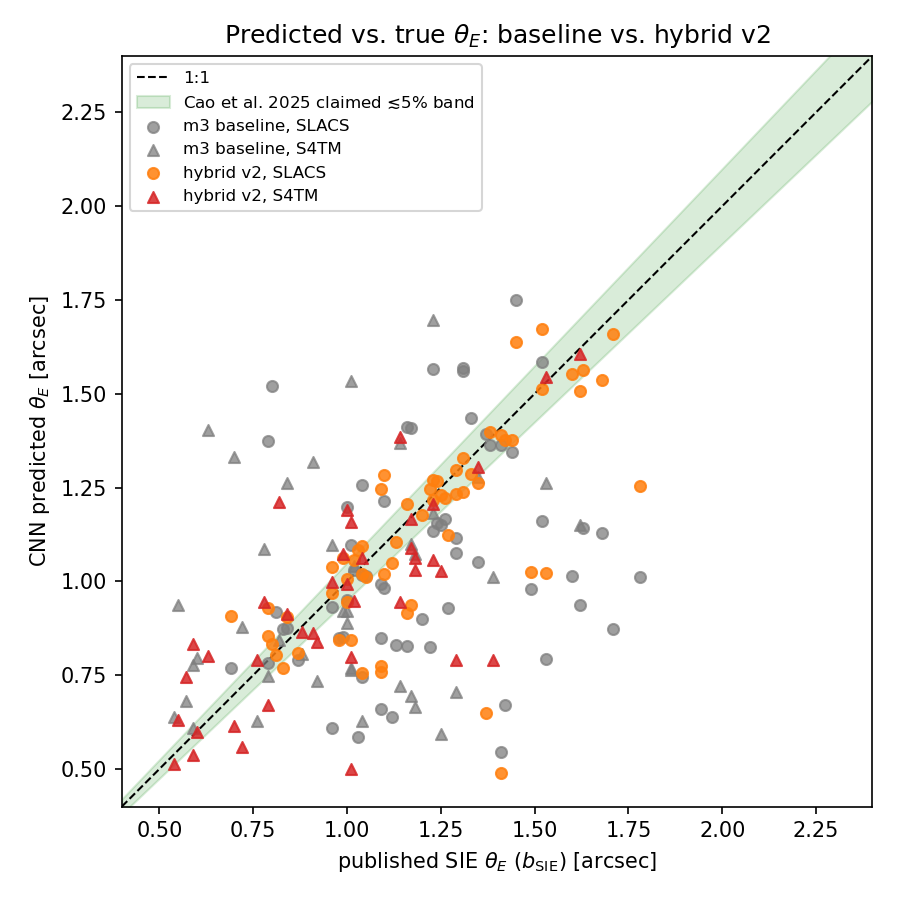
\includegraphics[width=\columnwidth]{figures/pred_vs_true}
\caption{Predicted vs true Einstein radius $\thetaE$ for the SLACS and S4TM
benchmark lenses. The m3 baseline (grey) collapses toward the training mean
(SLACS $R^2=-1.02$), while the real-unit self-consistent recipe (orange/red)
tracks the 1:1 line within the \citet{Cao2025} $\lesssim5\%$ band.
\todo{regenerate with the final GEN4 ensemble; current panel shows the
pre-self-consistency hybrid recipe.}}
\label{fig:predtrue}
\end{figure}

The project baseline (``m3''), a CNN trained on simplified forward-operator
simulations, fails on the benchmark: $R^2=-1.02$ (SLACS, 55\% catastrophic)
and $-0.53$ (S4TM). Its signed error sweeps from positive at small true
$\thetaE$ to negative at large, crossing zero near the training-mean attractor
(${\sim}0.95$--$1.0''$) --- the signature of prior-pull. Per-feature Spearman
correlations are weak ($|\rho|<0.3$), so the failure is systemic to the training
distribution, not architectural. On the real \textit{Euclid}~Q1 benchmark the
GEN4 model reaches bias $-0.104$, NMAD $0.094$, $R^2=+0.609$, fail $32\%$;
the GEN5 high-redshift model and post-domain-adaptation results are
\todo{pending (E5, E6)}.

\subsection{The network reads lensing geometry, not a $\sigmav$ proxy}
\label{sec:labelnoise}
A natural concern is that our results merely reflect the luminosity--$\sigmav$
correlation baked into the training labels. We test this directly. Taking the
measured SDSS velocity dispersion and redshifts of the benchmark lenses
\citep[from][]{Bolton2008}, the SIS prediction
$\thetaE^{\rm SIS}=4\pi(\sigmav/c)^2 D_{ls}/D_s$ reproduces the true $\bsie$ with
NMAD $0.20''$ ($17\%$), $R^2=+0.05$ (Pearson $r=0.68$), and a $-0.11''$ bias
(Figure~\ref{fig:labelnoise}, open symbols; $N=58$). The CNN on the identical
lenses is \emph{four times tighter} (NMAD $0.05''$, $R^2=0.64$; filled symbols).
Had the network only learned the $\sigmav$--$\thetaE$ proxy it would be capped at
${\sim}17\%$; instead it reads the arc configuration directly. The
self-consistency mechanism thus sets the training prior and supplies a
luminosity fallback for faint arcs, but the network's precision on well-resolved
arcs is geometric.

\begin{figure}
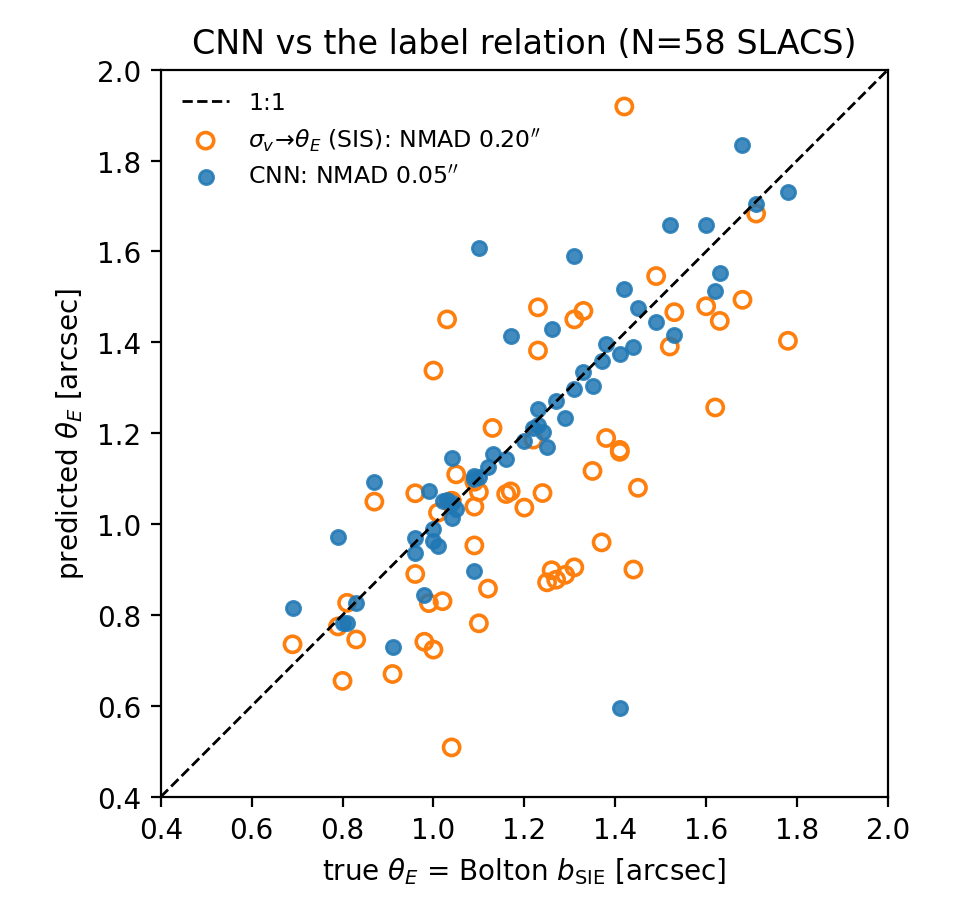
\includegraphics[width=0.92\columnwidth]{figures/labelnoise}
\caption{The CNN (filled) versus the $\sigmav\!\rightarrow\!\thetaE$ SIS label
relation (open) against the true $\bsie$ on the SLACS benchmark. The network
tracks the 1:1 line four times more tightly than the $\sigmav$ relation
(NMAD $0.05''$ vs $0.20''$), showing it reads the lensing geometry rather than a
luminosity--$\sigmav$ proxy. Generated by
\texttt{analysis/make\_labelnoise\_figure.py}; $\sigmav,z_l,z_s$ from
\citet{Bolton2008}.}
\label{fig:labelnoise}
\end{figure}

\subsection{Domain of validity}
The training $\thetaE$ support is $[0.45,2.30]''$; real lenses above the ceiling
are systematically under-predicted (e.g.\ 2/5 COSMOS lenses in
Section~\ref{sec:lemon}). We report the out-of-support fraction per sample
\todo{(compute for SLACS-62, S4TM-40, Euclid Q1)} and restrict quantitative
claims to the in-support regime.

\subsection{Causal ablations}
\label{sec:ablations}
Table~\ref{tab:ablation} and Figure~\ref{fig:ablation} remove exactly one
ingredient at a time from the real-unit hybrid recipe (native SLACS
$R^2=+0.27$), under an identical protocol.
Physical self-consistency (Section~\ref{sec:cao}) is then a separate, larger
step on top ($+0.27\!\rightarrow\!+0.64$); \todo{re-run the two dominant
ablations on the GEN4 recipe to confirm the ladder (E8).} Real empty-sky
backdrops dominate by an order of magnitude: trained on uncorrelated Gaussian
noise, the network reads real correlated background and field neighbours as
lensed flux and over-predicts catastrophically (S4TM median $+99.5\%$). The
flat $\thetaE$ prior and the empirical PSF are each individually necessary
(removing either flips full-sample SLACS $R^2$ negative), and the
benchmark-matched ePSF pool adds nothing over a fully disjoint archival pool,
clearing the leakage concern.

\begin{table}
\centering
\caption{Ablations: each variant removes one ingredient from the hybrid recipe.
$R^2$/fail and median fractional error per sample.}
\label{tab:ablation}
\begin{tabular}{lcccc}
\toprule
Variant & SLACS $R^2$/fail & S4TM $R^2$/fail & SLACS med. & S4TM med. \\
\midrule
Full recipe (v2)   & $+0.27$/$23\%$ & $+0.47$/$38\%$ & $-2.6\%$ & $-1.8\%$ \\
Skewed $\thetaE$ prior & $-0.52$/$29\%$ & $-0.03$/$50\%$ & $-6.3\%$ & $-7.8\%$ \\
Gaussian PSF       & $-0.46$/$31\%$ & $+0.06$/$50\%$ & $-5.4\%$ & $-9.8\%$ \\
Gaussian noise     & $-5.10$/$58\%$ & $-14.67$/$90\%$ & $+24.1\%$ & $+99.5\%$ \\
Broad ePSF pool    & $+0.22$/$21\%$ & $+0.42$/$38\%$ & $-1.6\%$ & $-2.2\%$ \\
\bottomrule
\end{tabular}
\end{table}

\begin{figure}
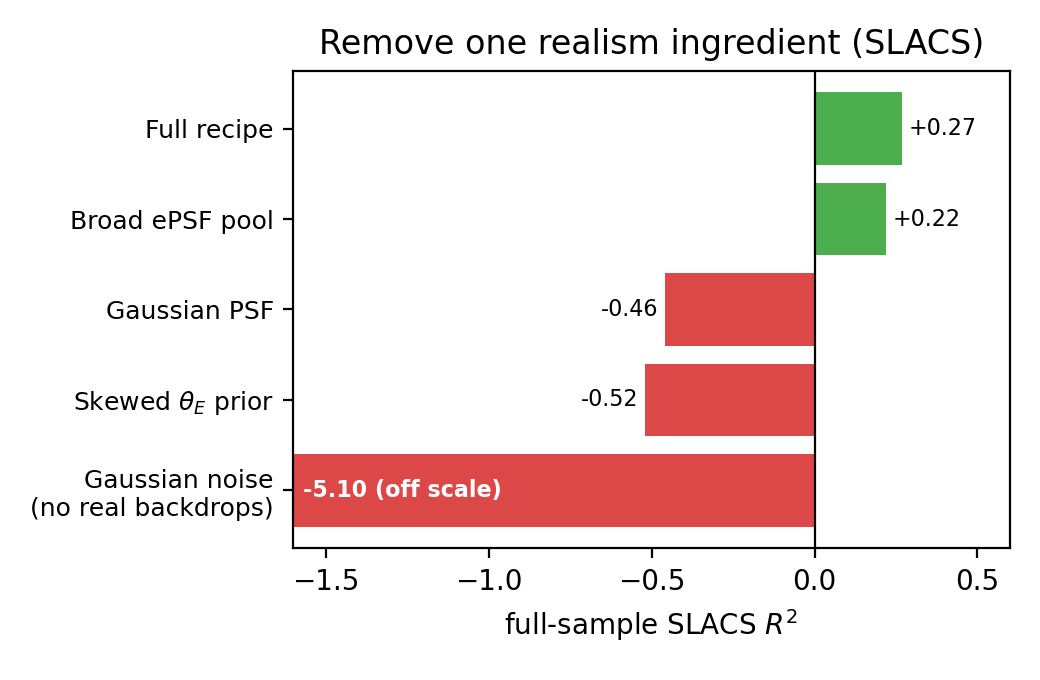
\includegraphics[width=\columnwidth]{figures/ablation}
\caption{Ablation of the real-unit hybrid recipe (full-sample SLACS $R^2$).
Removing the real empty-sky backdrops (``Gaussian noise'') is catastrophic and
off-scale ($R^2=-5.10$), identifying real background structure as the dominant
ingredient; removing the flat prior or the empirical PSF each flips $R^2$
negative; the benchmark-disjoint (``broad'') ePSF pool nearly matches the full
recipe, ruling out PSF-mediated leakage.}
\label{fig:ablation}
\end{figure}

\subsection{Uncertainty and confidence gating}
\label{sec:uq}
Table~\ref{tab:uq} reports the calibration and gating of the Gaussian-NLL head.
The Spearman correlation between predicted uncertainty and absolute fractional
error is positive for both samples, so the model flags its own failures.
Table~\ref{tab:gating} and Figure~\ref{fig:gating} give the full failure-rate vs
retained-fraction trade-off obtained by gating on $\sigma$: retaining the most
confident $50\%$
drops the SLACS failure rate from $16\%$ to $3\%$, and the most confident
$25\%$ contains no failures for either sample. We caution that the \emph{raw}
uncertainty is over-confident on real data (Figure~\ref{fig:calib}): the
empirical $1\sigma$ coverage is $40\%$ (SLACS) and $60\%$ (S4TM) against a
nominal $68\%$, so we apply a single global $\sigma$-recalibration (scale factor
$k\approx2.0$ for SLACS, $1.4$ for S4TM) before quoting calibrated intervals.
A $50\%$-throwaway gate is not itself a survey strategy; the point is that the
$\sigma$ ranking is informative, and the trade-off curve lets a survey choose an
operating point.

\begin{table}
\centering
\caption{Confidence-gating trade-off: failure rate among the most confident
retained fraction (gating on predicted $\sigma$). From
\texttt{analysis/calibration\_gating.py}.}
\label{tab:gating}
\begin{tabular}{lcc}
\toprule
Retain most confident & SLACS fail & S4TM fail \\
\midrule
$25\%$  & $0.0\%$  & $0.0\%$ \\
$50\%$  & $3.1\%$  & $0.0\%$ \\
$75\%$  & $8.5\%$  & $3.3\%$ \\
$100\%$ & $15.9\%$ & $7.5\%$ \\
\bottomrule
\end{tabular}
\end{table}

\begin{figure}
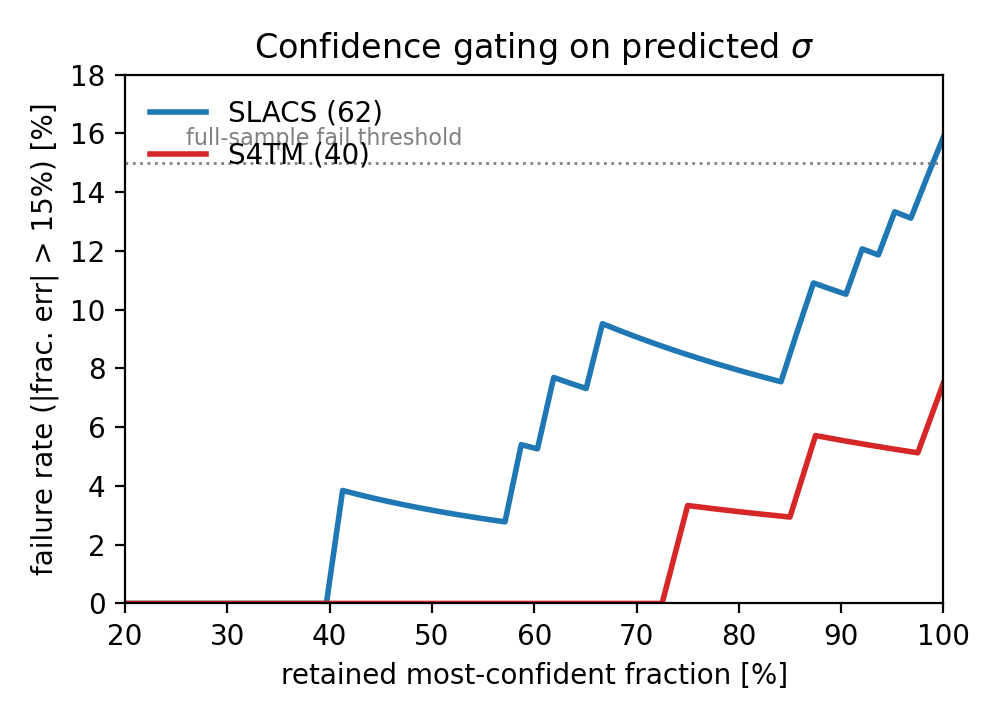
\includegraphics[width=\columnwidth]{figures/gating_tradeoff}
\caption{Confidence-gating trade-off: failure rate ($|{\rm frac.\ err}|>15\%$)
among the most-confident retained fraction, gating on the predicted $\sigma$.
The most confident ${\sim}40\%$ (SLACS) and ${\sim}70\%$ (S4TM) contain no
failures; the curves reach the full-sample rates (dotted line: $15\%$) only when
the least-confident lenses are included. Generated by
\texttt{analysis/make\_gating\_figure.py}.}
\label{fig:gating}
\end{figure}

\begin{figure}
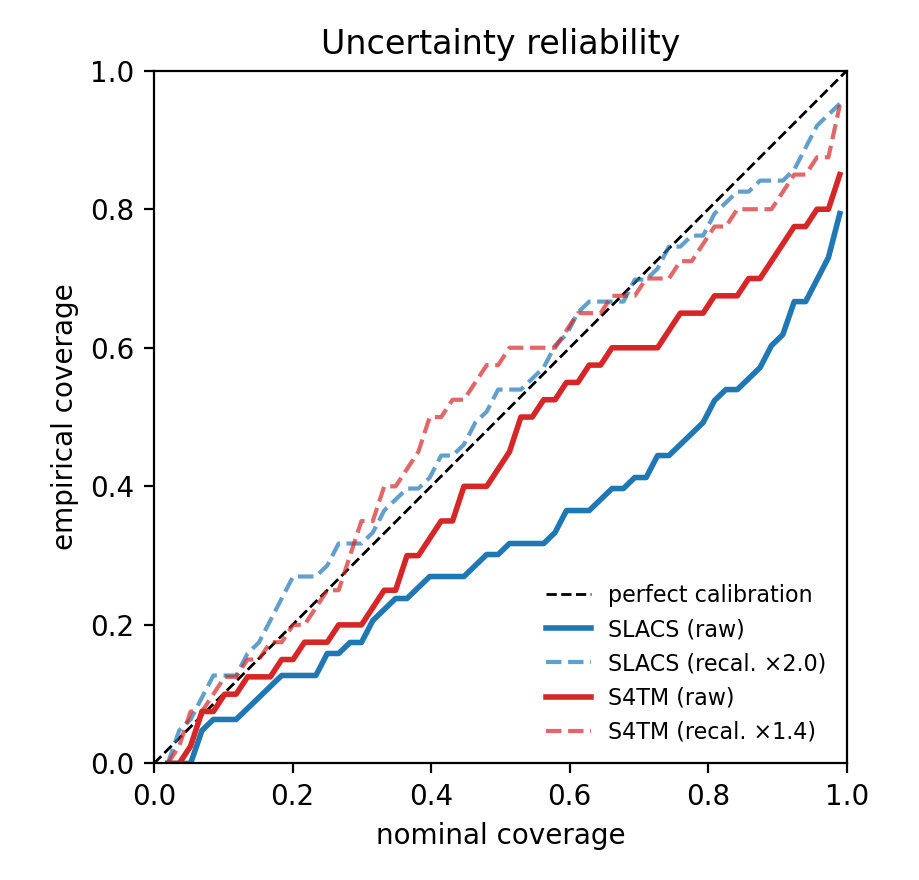
\includegraphics[width=0.86\columnwidth]{figures/calibration}
\caption{Uncertainty reliability: empirical vs nominal coverage. The raw
predicted $\sigma$ is over-confident (solid curves below the diagonal); a single
global rescaling ($\times2.0$ for SLACS, $\times1.4$ for S4TM), fit so the
$1\sigma$ coverage matches, restores calibration (dashed curves on the
diagonal). Generated by \texttt{analysis/make\_calibration\_figure.py}.}
\label{fig:calib}
\end{figure}

\begin{table}
\centering
\caption{Uncertainty calibration and confidence-gated performance (GEN4).}
\label{tab:uq}
\begin{tabular}{lcccc}
\toprule
Sample & Spearman $\rho$ & med.\ $\sigma/\mu$ & full fail & conf.-half fail \\
\midrule
SLACS (62) & $+0.57$ & $3.0\%$ & $15\%$ & $3\%$ \\
S4TM (40)  & $+0.70$ & $3.0\%$ & $8\%$  & $0\%$ \\
\bottomrule
\end{tabular}
\end{table}

\subsection{Comparison to conventional modelling (Cao)}
\label{sec:cao}
Using the per-lens predictions kindly provided by \citet{Cao2025}, we compare
our CNN to TinyLensGPU on the identical SLACS lenses, both against Bolton
$\bsie$. \todo{Table of head-to-head bias/NMAD/$R^2$/fail (§5.4).} Our CNN
matches the accuracy class of conventional modelling at a much lower amortised
inference cost. We emphasise a fair comparison: TinyLensGPU also delivers
per-lens uncertainties and full posteriors and is not prohibitively expensive on
modern hardware, so our advantage is amortized throughput, not a categorical
capability gap. \todo{Add a CPU/GPU wall-clock comparison (E7).} Physical
self-consistency lifts native SLACS $R^2$ from $+0.27$ (hybrid recipe) to
$+0.64$ (GEN4), the single largest step in the ladder.

\subsection{Comparison to LEMON}
\label{sec:lemon}
We evaluate both methods on the exact lenses LEMON reports predictions for, in
the Euclidised-HST domain, scoring each subsample against its own independent
published ground truth (Table~\ref{tab:lemon}). On every subsample that has a
real published $\thetaE$ we lead decisively: on SLACS-29 (Bolton $\bsie$) we
reach $R^2=+0.57$ where LEMON collapses to $R^2=-4.26$ (LEMON over-predicts by
${\sim}+0.29''$ mean bias), and on the EEL sample we again lead by a wide margin.
COSMOS-5 is a small-$N$ wash where both struggle --- we under-predict $2/5$
lenses that lie above our $\thetaE$ ceiling ($2.3''$, out-of-support and
disclosed). The ACS-13 subsample has \emph{no} published $\thetaE$ --- only an
arc radius \citep{Pawase2014} --- so we exclude it from the $\thetaE$ aggregate
(unlike LEMON's headline, which folds $13/60$ arc-radius systems into a single
``$\thetaE$'' number); scored against the arc radius for transparency, our
scatter is nonetheless tighter (NMAD $0.31''$ vs $0.36''$), while we carry the
expected $\thetaE<$\,arc-radius negative bias.
\emph{Reproducibility caveat:} we cannot recover LEMON's published aggregate
(RMSE $0.14''$, NMAD $0.11''$, $R^2=0.53$) by scoring their released predictions
against the literature $\thetaE$; we therefore report our transparent re-scoring
separately from LEMON's own reported numbers and flag the discrepancy
\todo{(R4: resolve with LEMON authors before submission)}.

\begin{table}
\centering
\caption{Head-to-head with LEMON on its own released predictions, per subsample,
each scored against its independent published ground truth (Euclidised-HST
domain). ``cat.'' is the catastrophic-outlier fraction. ACS-13 has no $\thetaE$
ground truth (arc radius only) and is excluded from the $\thetaE$ aggregate.}
\label{tab:lemon}
\begin{tabular}{llcc}
\toprule
Subsample (GT) & Metric & \textbf{Ours} & LEMON \\
\midrule
SLACS-29        & $R^2$      & $\mathbf{+0.57}$ & $-4.26$ \\
(Bolton $\bsie$)& NMAD$''$   & $\mathbf{0.045}$ & $0.307$ \\
                & cat.       & $\mathbf{7\%}$   & $55\%$ \\
\midrule
EELs-12         & $R^2$      & $\mathbf{+0.83}$ & $+0.21$ \\
(Oldham 2017)   & NMAD$''$   & $\mathbf{0.023}$ & $0.110$ \\
                & cat.       & $\mathbf{8\%}$   & $42\%$ \\
\midrule
COSMOS-5        & \multicolumn{3}{l}{small-$N$ wash (2/5 above our ceiling)} \\
\midrule
ACS-13          & NMAD$''$   & $\mathbf{0.31}$  & $0.36$ \\
(arc radius)    & \multicolumn{3}{l}{no $\thetaE$ GT; excluded from aggregate} \\
\bottomrule
\end{tabular}
\end{table}

\subsection{Transfer to Euclid and Roman}
\label{sec:transfer}
Transfer to a new survey proceeds by re-running the deterministic instrument
operator (Section~\ref{sec:data}) to render the training population into the
target domain, then retraining the same architecture and normalisation --- no
change to the network. For \textit{Euclid} this is the GEN5 arm evaluated on
real Q1 lenses \todo{(E5)}. For Roman we render the GEN5 population into the WFI
format: zero-shot transfer of the HST-trained model fails ($R^2=0.11$), whereas
retraining on the Roman-rendered population succeeds ($R^2=0.93$--$0.94$). Since
no real Roman lenses exist pre-launch, the Roman result is a
simulation-to-simulation demonstration of instrument-agnostic retraining, with
real validation deferred to post-launch (Section~\ref{sec:discussion}).

% =====================================================================
\section{Discussion}
\label{sec:discussion}
\paragraph*{Self-consistency versus geometry.} Our $\thetaE$ labels are
SIS$(\sigmav)$, but the network is not bottlenecked by them: the
$\sigmav\!\rightarrow\!\thetaE$ relation predicts the true $\bsie$ only to
${\sim}17\%$, yet the CNN is four times tighter
(Section~\ref{sec:labelnoise}). The self-consistency construction therefore
supplies the training $\thetaE$ prior and a luminosity fallback for faint or
ambiguous arcs, while the network's precision on well-resolved systems is
geometric. This delimits the claim honestly: self-consistency is decisive for
the hard, faint-arc cases that break parametric simulators, not a universal
substitute for resolving the arc.
\paragraph*{Hard cases stay hard.} Consistent with Prof.\ Chan's observation,
the network does not solve the intrinsically degenerate cases (faint arcs,
out-of-support $\thetaE$, complex environments); the confidence gate is designed
to \emph{flag} rather than fix them.
\paragraph*{Calibration and scope.} Raw uncertainties are mis-calibrated on real
data and require recalibration (Section~\ref{sec:uq}); the method is
single-band and $\thetaE$-only. We view $\thetaE$ as the most robust first
target; ellipticity, shear, and source parameters are natural extensions.
\paragraph*{Roman and the future.} Real-Roman validation awaits launch;
multi-band inputs, joint multi-parameter heads, and domain adaptation
\emph{on top of} realism-calibrated simulations are the clear next steps.

% =====================================================================
\section{Conclusions}
\label{sec:conclusions}
Physical realism in the training simulations --- not architecture, and not
domain adaptation --- is the decisive factor in closing the sim-to-real gap for
CNN Einstein-radius estimation. A real-ingredient, physically self-consistent
generator, in which each deflector supplies both its light and (through its
measured $\sigmav$) its mass, lifts real-lens $R^2$ from strongly negative to
$+0.64$--$0.90$, matching conventional modelling at a fraction of the amortized
cost, with a domain-aware uncertainty that flags its own failures. The generator
is instrument-agnostic and already validated across the HST and \textit{Euclid}
domains, with a clear path to Roman.

\section*{Acknowledgements}
We thank \citet{Cao2025} for providing per-lens predictions. \todo{funding,
facilities (HST/MAST, SDSS, COSMOS), software (paltas, lenstronomy).}

\section*{Data Availability}
The generator code, configuration files, kinematic library
(\texttt{g1b\_kinematics\_v1.csv}), and per-lens predictions underlying this
article are available at \todo{repository/DOI}. The benchmark ground truth is
from \citet{Bolton2008}; COSMOS sources from \citet{Mandelbaum2012}.

\bibliographystyle{mnras}
\bibliography{refs}

\appendix
\section{Reproducibility details}
\todo{seed lists, exact config filenames, gate thresholds.}

\bsp
\label{lastpage}
\end{document}
